%-----------------------------------------------------------------------------
% Schriftgr��e, Layout, Papierformat, Art des Dokumentes
%-----------------------------------------------------------------------------
\documentclass[12pt,					% Grundschriftge
							 oneside,			% einseitiges Dokument
							 a4paper,			% Papiergr��e
							 halfparskip,		% Einzug bei einem Absatz
							 liststotoc,			% Verzeichniss (Abbildungen erc.) in das Inhaltverzeichnis
							 bibtotoc,			% Literaturverzeichnis ins Inhaltverzeichnis
							 fleqn,				% Mathematische Formeln linksb�ndig darstellen
							 pointlessnumbers]	% Punkt am Ende der Nummerierung des Inhaltsverzeichnisses 													entfernen
							 {scrreprt}

%-----------------------------------------------------------------------------
% Konstanten festlegen
%-----------------------------------------------------------------------------
\newcommand{\VerfasserJ}{Josef Prothmann}
\newcommand{\EmailJ}{j.prothmann@stud.hs-wismar.de}
\newcommand{\GeburtstagJ}{16. Dezember 1998}
\newcommand{\GeburtsortJ}{Dannenberg/ Elbe}

\newcommand{\Titel}{Implementierung einer Fernsteuerung für einen 3D gedrukten Roboterarm über einen Rasberry PI 3}
\newcommand{\Betreuer}{Prof. Dr. H. Litschke}



\newcommand{\blankpage}{
%	\newpage
%	\thispagestyle{empty}
%	\mbox{}
	\newpage
}

%-----------------------------------------------------------------------------
% verwendete Pakete
%-----------------------------------------------------------------------------
\usepackage[utf8]{inputenc}		% Zeichkodierung , Umlaute erlauben
\usepackage[T1]{fontenc}				% Wahl des Fonts, bzw. der Kodierung
\usepackage[english,ngerman]{babel}		% neue deutsche Rechtschreibung verwenden
\usepackage{graphicx}					% erm�glicht das Einbinden von Grafiken, sehr wichtig!
\usepackage{fancyhdr}					% f�r formatierte Kopf- und Fu�zeilen
\usepackage{setspace}					% Package zum Kontrollieren von Leerr�umen
\usepackage{subfigure}					% erweiterte Darstellung von Bildern
\usepackage{listings}					% M�glickeit zum Anzeigen von Quelltexten
\usepackage{color,moreverb}				% Farben
\usepackage{lmodern}					% bietet neuere Schriften, sieht besser aus im Acrobat Reader
\usepackage{amsmath,amssymb}			% erweiteter Formelsatz und zus�tzliche Mathe-Symbole
\usepackage{booktabs}					% professionelle, typographisch richtige Tabellen
\usepackage{cite}						% f�r LibTex
%\usepackage{shortvrb}					% f�r Quellcode mit \begin{verbatim}
\usepackage[binary-units=true]{siunitx}	% Darstellung von Si-Einheiten
%\usepackage{pdfpages}					% pdf-Seiten einbinden
\usepackage{enumitem}					% custom itemiziation





%-----------------------------------------------------------------------------
% Fu�notennummerierung nicht f�r jedes kapitel zur�cksetzen
%-----------------------------------------------------------------------------
\usepackage{chngcntr}
\counterwithout{footnote}{chapter}

%-----------------------------------------------------------------------------
% Einstellungen der Seitenr�nder
%-----------------------------------------------------------------------------
\usepackage[left=3cm,						% linker Rand
						right=3cm,			% rechter Rand
						top=1.5cm,			% oberer Rand
						bottom=1.5cm,		% unterer Rand
						includeheadfoot,	% bezieht die Kopf- und Fu�zeile mit ein
						bindingoffset=0cm]	% Bundsteg
						{geometry}



%-----------------------------------------------------------------------------
% Daten f�r die Titel des Artikels
%-----------------------------------------------------------------------------
\title{Praktikumsbericht}
\author{\Verfasserj}
\date{\today{}}

%-----------------------------------------------------------------------------
% Metadaten in pdf einf�gen
%-----------------------------------------------------------------------------
\usepackage[pdftex,
						pdfauthor={\VerfasserJ},									% Name des Autors
						pdftitle={\Titel},										% Name der Arbeit
						pdfcreator={MiKTeX, LaTeX with hyperref and KOMA-Script},	% Von was erzeugt
						pdfsubject={Praktikumsbericht},							% Was f�r eine Arbeit ist es
						pdfkeywords={\Titel},
						plainpages=false,
						hypertexnames=false,
						pdfpagelabels]{hyperref}

%-----------------------------------------------------------------------------
% Schriftarten anpassen
%-----------------------------------------------------------------------------
\setkomafont{sectioning}{\rmfamily\bfseries}			% Titelzeilen
\setkomafont{caption}{\small}							% Schrift f�r Caption
\setkomafont{captionlabel}{\sffamily\bfseries\small}	% Schrift f�r 'Abbildung'
\setkomafont{chapterentry}{\small\bfseries}				% Schrift f�r Inhaltsverzeichnis
\setkomafont{chapter}{\large\bfseries}					% Schrift f�r Kapitel
\setkomafont{section}{\normalsize}						% Schrift f�r Section
\setkomafont{subsection}{\normalsize}					% Schrift f�r Subsection
						



				
%-----------------------------------------------------------------------------
% Kopf- und Fusszeile bestimmen
%-----------------------------------------------------------------------------
\pagestyle{fancy}	
\fancyhf{}												% alle Felder l�schen
\fancypagestyle{plain}{}

% Kopfzeile rechts bzw. au�en
\fancyhead[R]{\nouppercase{\leftmark}}
% Linie oben
\renewcommand{\headrulewidth}{0.5pt}
% Fu�zeile rechts bzw. au�en
\fancyfoot[R]{\thepage}
%-----------------------------------------------------------------------------

%-----------------------------------------------------------------------------
% Begin des Dokuments
%-----------------------------------------------------------------------------

\begin{document} 						% Beginn des Dokumentes

	\renewcommand\lstlistingname{Code}
	\renewcommand\lstlistlistingname{Codeverzeichnis}
	
	%% Titel
	\begin{titlepage}
		\setlength\headsep{-5mm}
		\begin{figure}[!h]
			\begin{minipage}{0.8\textwidth}
				\textbf{Hochschule Wismar} \\
				University of Applied Sciences \\
				Technology, Business and Design \\
				Fakultät für Ingenieurwissenschaften, Bereich EuI \\
			\rule{\textwidth}{0.5pt}
			\end{minipage}
			\begin{minipage}[r]{0.1\textwidth}
				\begin{flushright}
					
\includegraphics[height=6\baselineskip]{pictures/HS-Wismar_Logo-FIW_2010-01.jpg}
				\end{flushright}
			\end{minipage}
		\end{figure}
		\vspace*{6cm}
		\begin{center}
			\Huge
			\textbf{Semesterarbeit im Fach\\ User Interfaces} \\
			\vspace{2cm}
			\large \Titel
			\begin{table*}[b]
				\begin{tabular}{rl}
					
					Eingereicht am: &\today \\
					\\
					& \VerfasserJ \\ 
					& geboren am \GeburtstagJ \\ 
					& Email: \EmailJ \\
					\\

					Betreuer: & \Betreuer \\

				\end{tabular}
			\end{table*}
		\end{center}
	\end{titlepage}

	\onehalfspacing 					% 1 1/2-zeilig (package 'setspace')
	
\pagenumbering{roman}

	%-----------------------------------------------------------------------------
	% Inhaltsverzeichnis
	%-----------------------------------------------------------------------------	
	\pdfbookmark[1]{Inhaltsverzeichnis}{toc}	% Inhaltsverzeichnis zu den Lesezeichen hinzuf�gen
	%\singlespacing 						% 1-zeilig
	
	%\onehalfspacing 					% 1 1/2-zeilig (package 'setspace')
\section*{Abstrakt}
Diese Arbeit beschäftigt sich mit der Implentierung eines User Interfaces für einen Roboterarm, welcher von einem 3D Drucker hergestellt und über einen Server mit einer Android Applikation zur Fernsteuerung verbunden ist.
\section*{Abstract}
This thesis is facing the implementation of an user interface for an robotic arm wich is crafted by a 3D printer and is connected to a server while it is remote controlled by an android application.
\tableofcontents
\pagenumbering{arabic} 					% Inhaltverzeichnis einf�gen
	%-----------------------------------------------------------------------------
	% Hauptteil
	%-----------------------------------------------------------------------------	

\chapter{Einleitung}
Der Benutzerschnittstelle, oder auf Englisch, dem \glqq{}User Interface\grqq{}, wird zunehmend Aufmerksamkeit gewidmet. Dies resultiert aus der laufenden Digitalisierung von Prozessen und der stetigen Übernahme der Computern und Maschinen von menschlichen Aufgaben. Denn selbstverständlich muss zwischen dem Staubsaugroboter aus dem Wohnzimmer oder dem Industrieroboter in der Produktioneine eine Benutzerschnittstelle (HMI\footnote{engl. Human-Machine Interface}) geschaffen werden, damit eine Kontrolle und eine Zuweisung dieser Aufgaben stattfinden kann. \\
In diesem Projekt wurde eine Benutzerschnittstelle für einen Roboterarm entwickelt, mit dem sich dieser steuern lässt. 
\chapter{Grundlagen}
\section{Hardware Komponenten}
\section{3D - Druck}
\section{Android}
Android ist ein von Google Inc. entwickeltes und das meist verbreiteste Betriebsystem auf dem deutschen Markt\footnote{Stand März 2020 laufen ca. 80\% der verfügbaren Geräte mit einem Android Betriebssytem -\textit{Quelle: Statista.com, \glqq{}Vergleich der Marktanteile von Android und iOS am Absatz von Smartphones in Deutschland von Januar 2012 bis März 2020\grqq{}, 03.06.2020}\cite{Tenzer2020}}. Mittlerweile findet es nicht mehr nur in Smartphones, sondern auch in Smartwatches, Tablets und in Fernsehern Verwendung. Die App wurde auf der Version 8.1 (Oreo) entwickelt, ist aber trotzdem für aktuellere Versionen verfügbar.
\chapter{Konzeption}
Bei dem Entwurf des Graphical User Interfaces (GUI), wurde sich an gängien Fernsteuerungen aus der Spielebranche orientiert. Auf der Linken, sowie auf der rechten, unteren Seite des Displays, lässt sich die Position des Armes im dreidimensionalen Raum (3D) steuern. im oberen Bereich der Anwendung befinden sich Konfigurationspunkte sowie der \glqq{}Switch\grqq{}\footnote{Ein Switch ist in Android ein Kippschalter mit 2 Zuständen}, welcher Steuern des Greifers übernimmt. Die App sollte nur im \glqq{}Landscape\grqq{}-Modus, ausführbar sein. Dabei wurde Wert auf das Einhalten von aktuellen Konventionen, wie einem Settings Menü zum Festlegen von Serverport und -ip und CISCO Standart Symbolen wie dem Netzwerk-Symbol geachtet. Des Weiteren wurde mit dem Erstellen von eigenen Scaleable Vector Graphics (SVG) die Intiutivität unterstützt und eine missverständliche Nutzung der Applikation ausgeschlossen.\\ \\ \\ \\ \\ \\ \\


Hier nun Konzeptidee vom Arm und Servercode

\chapter{Implementierung}	
Für die Entwicklung einer nativen Android App wird die Entwicklungsumgebung Android Studio benötigt. Des Weiteren wird für die Softwareversionsverwaltung auf die Plattform Github zurückgegriffen, wo der Quellcode des Projektes dokumentiert ist\footnote{https://github.com/JoProt/User-Interface-Project}. Aus dem Grund, dass die Verbindung zu dem Roboter Arm über das Internet realisiert wurde, ist es notwendig in dem Manifest der Applikation die Internetberechtigung zu erteilen. \\
\begin{lstlisting}
<uses-permission android:name="android.permission.INTERNET" />
\end{lstlisting}

Damit ist es möglich auf das mobile Netz des Smartphones zuzugreifen. Um eine Verbindung aufzubauen, benötigt der Client, in diesem Fall die App, die Adresse und den Port des Hosts, in diesem Fall der Server auf dem Raspberry Pi. \\
Die Parameter für die Verbindung (IP und Port des Hosts), lassen sich dynmaisch (zur Laufzeit) in der App einsehen und anpassen. Dadurch ist es in der Theorie möglich, mehrere Roboter nacheinander zu steuern. 
Damit das ankommende Signal, welches von die Knöpfen und der Switch senden korrekt interpretiert wird, sendet die App einen eindeutigen, einstelligen Integer Code. Dadurch lassen sich die Bewegungen der Motoren durch den korrekten Knopf in der App abbilden. \\ \\
Da Pfeile als Bewegungsindikatoren im 3D Raum leicht missverstanden werden können, wurden eigene SVGs erstellt, welche die Bewegung des Arms verdeutlichen. \\
\begin{figure}[h]
	\centering
	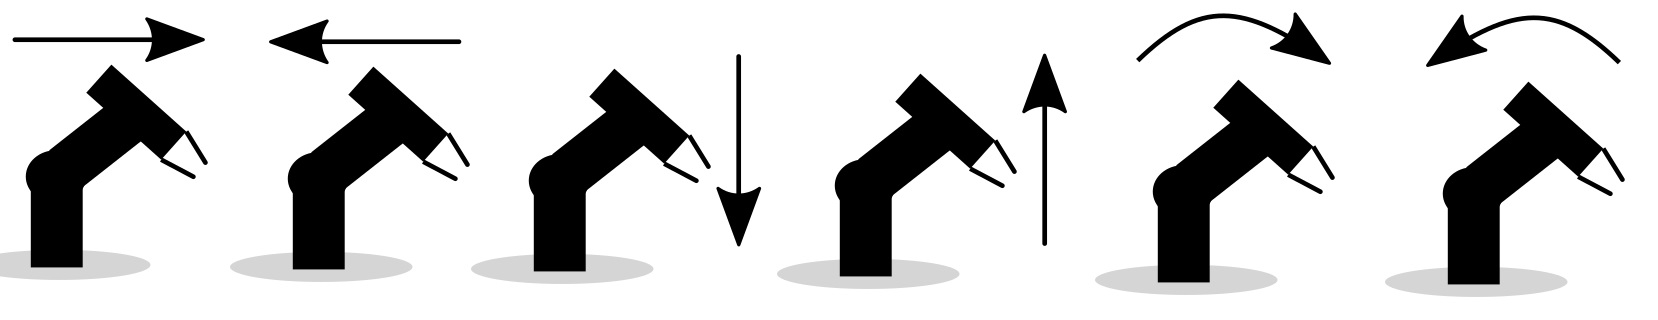
\includegraphics[scale=0.3]{pictures/robissvg.jpg}
	\caption{SVG der Knöpfe aus der App \textit{- Quelle: Eigene Darstellung}}
\end{figure}
\newpage
In Abbildung 4.1 sind die einzelnen Grafiken für die jeweilige Bewegung des Roboters aufgelistet, wobei $\leftarrow$ und $\rightarrow$ für Steuerung auf einer horizontal Linie, $\uparrow$ und $\downarrow$ für vertikale Bewegungen und $\curvearrowleft$ und $\curvearrowright$ für Bewegung um die eigene Hochachse verantwortlich sind.
\chapter{Zusammenfassung}	
In diesem Projekt haben wir uns mit den Grundlagen der Entwicklung eines User Interfaces auseinandergesetzt und eine ansprechende und intuitiv zu bedienende App entwickelt. Mit Hilfe unseres Wissens aus weiteren Modulen, wie zum Beispiel \glqq{}Programmierung Mobiler Endgeräte\grqq{} und \glqq{}Echtzeit- und Netzwerktprogrammierung\grqq{}, war es uns möglich eine Android Anwendung zu schreiben um einen 3D gedruckten Roboter Arm zusteuern. 
\\
In der Zeit der Digitalisierung, in der Computer immer mehr Teil unseres Alltags werden ist es das Ziel, dass die Maschinen für den Menschen eine Arbeitserleichterung und keine Last werden. Desshalb ist es umso wichtiger, mit einem qualitativem User Interface zu arbeiteten. Dieses vergleichsweise kleine Projekt hat uns gezeigt wie aufwendig der Prozess der Gestaltung einer hochwertigen Oberfläche ist.\\ \\
Gerade dann, wenn eine Anwendung veröffentlicht und von mehreren Menschen genutzt wird, ist es wichtig, dass es das Leben erleichtert und nicht verkompliziert.
\pagenumbering{roman}

	%-----------------------------------------------------------------------------
	% Literaturverzeichnis einf�gen, 
	% Nutzung der BibTeX-Technologie --> literatur.bib 
	%-----------------------------------------------------------------------------

	
	\bibliographystyle{unsrtdin}		%  Stil des Literaturverzeichnisses (hier nach DIN 1505)
	\bibliography{literatur}			% gibt Datei mit der Literatur an
	
	\nocite{*}						% damit alle in der DB enthaltende Eintr�ge bearbeitet werden
	

	%-----------------------------------------------------------------------------
	% Verzeichnisse
	%-----------------------------------------------------------------------------
	\listoffigures						% Bildverzeichnis einf�gen

	%-----------------------------------------------------------------------------
	% Anhang
	%-----------------------------------------------------------------------------	
	\appendix
	% Auch hier sind Gliederungen aller \chapter, \section
	

	%-----------------------------------------------------------------------------
	% Selbstst�ndigkeitserkl�rung
	%-----------------------------------------------------------------------------	
	\chapter*{Selbstst\"andigkeitserkl\"arung}
	\addcontentsline{toc}{chapter}{Selbstst\"andigkeitserkl\"arung}
	\rhead{Selbstst\"andigkeitserkl\"arung} % rechts oben in der Kopfzeile Chapter darstellen
	Hiermit erkl\"aren wir, dass wir die hier vorliegende Arbeit selbstst\"andig,
	ohne unerlaubte fremde Hilfe und nur unter Verwendung der aufgef\"uhrten
	Hilfsmittel angefertigt haben.

	\begin{tabular}{p{10cm}p{13cm}}
		\\
  		\\
  		\\
  		\\
  		Wismar, den \today \\
  		---------------------------------------  & ------------------------------ \\
  		Ort, Datum & Unterschrift
	\end{tabular}
	

\end{document}							% Ende des Dokuments
%-----------------------------------------------------------------------------
